
\chapter{\gls{BNP} inference within \glspl{PPL}} \label{BNP_PPL}
In this chapter we focus on the task of performing inference within a \gls{PPL} for models with an infinite dimensional component, also called \gls{BNP} models.

For now we have restricted ourselves to infinite mixture models, but we hope that our framework will enable efficient sampling for other \gls{BNP} models such as the infinite \acrlong{HMM}. We have also focused our study on sampling methods, but \acrlong{VI} is considered in Section \ref{BNP_VI}.

\textcolor{red}{Stochastic Memoization perspective ??}
An interesting perspective of Discrete Random Probability Measure is through \textit{stochastic memoization} \footnote{\url{https://probmods.org/chapters/12-non-parametric-models.html}}.
First let's recall what is the usual (deterministic) memoization.
For instance with the \gls{DP}, with $\alpha = 0$ we recover a deterministic memoization whereas with $\alpha \rightarrow \inf$ there is no memoization at all.

\textcolor{red}{Useful ?}
-> Urn: posterior predictive distribution of $X_{k+1}$ given $X_0, \dots, X_{k}$
CRP: simple sufficient statistics, but in general not nice like that
All marginal samplers: Urn distributions, involve complicated integral (can sometimes introduce auxiliary variables)

Urn: marginalized out the random -> only partition left
Stick-breaking: hybrid-case, lazely instanciate our observation once they are drawn from it, sized-biased permutation

\section{Recursion is key}

In \glspl{PPL}, to transform a variable in a random variable, one only needed to write \texttt{x = sample(Dist(parameters))}. Then the posterior distribution (given some observations) of \texttt{x} will automatically be performed during the inference scheme.
The Bayesian setting thus naturally fits the framework of \glspl{PPL}.
Yet, we believe that there is more  than just a connection between Bayesian inference and \glspl{PPL}, but that there is also a connection between \acrlong{BNP} and High-order \gls{PPL}.

Working with \gls{BNP} models can be impossible because of the constraints of computers.
A \gls{NRM} $P$ can be written \cite{Kingman:1967kn} as
$$P = \sum_{k \ge 1}{\tilde{p}_k \delta_{X^\star_k}} $$
where $\left(\tilde{p}_k, X^\star_k \right)_{k \ge 1}$ is an infinite collection of weights and atoms.
Discrete probability measures with countable support such as \acrlongpl{NRM} cannot be represented in a computer in a naïve manner since a machine has finite memory.
Other representations of such objects must be used, if one hope to denote them in a program.

One key notion in programming languages which will be crucial is the concept of \textit{lazy evaluation} (or \textit{laziness}). It is an evaluation strategy which delays the evaluation of an expression until its value is needed and which also avoids repeated evaluations.
Lazy evaluation is often combined with \textit{memoization}, as described in \cite{Bentley:1982:WEP:539147}. After a function's value is computed for that parameter or set of parameters, the result is stored in a lookup table that is indexed by the values of those parameters; the next time the function is called, the table is consulted to determine whether the result for that combination of parameter values is already available. If so, the stored result is simply returned. If not, the function is evaluated and another entry is added to the lookup table for reuse.

Instead of hoping to construct the entire infinite sequence $\left({p}_k, X^\star_k \right)_{k \ge 1}$, we will only ``lazily'' sample $\left({p}_k, X^\star_k \right)$, i.e. when we need them.
Since we work with homogeneous \glspl{CRM}, the $\{X^\star_k\}_{k \ge 1}$ are independent and identically distributed according to the base distribution. Sampling the $(X^\star_k)_{k \ge 1}$ as we need them is therefore trivial. Yet, how could we lazily sample the $({p}_k)_{k \ge 1}$ ?
In Subsection \ref{DP}, we presented the stick-breaking process, a generative process for constructing of a size-biased permutation of $({p}_k)_{k \ge 1}$, denoted $(\tilde{p}_k)_{k \ge 1}$.
In Section \ref{SBS} we explore other generative processes, for more generic \gls{BNP} classes. For now, Let us recall the construction given by \cite{sethuraman94} for the stick-breaking process:


\begin{gather*}
V_1 \sim \text{Beta}(1, \alpha) \\
V_2 \sim \text{Beta}(1, \alpha) \\
\vdots \\
V_j \sim \text{Beta}(1, \alpha) \\
\vdots \\
\tilde{p}_k = V_k \prod_{j=1}^{k-1}(1-V_j) \ \ k= 1,2,\dots
\end{gather*}

Therefore, $\tilde{p}_k$ can be seen as the probability of the following sequence of outcomes: $k-1$ Bernouilli draws with respective probabilities $V_j \ , j=1,\dots,k-1$, all yield failure, and one last Bernouilli draw with probability $V_k$ yields success.
How can this be interpreted as a generative process on an infinite set of discrete outcomes ?
%With this insight so as to sample from a \gls{CRP}, or equivalently from a \gls{DP} with a base distribution on the natural numbers.
Imagine ``walking'' down the natural numbers in order, flipping a coin with weight $V_k$ (also called stick) for each one; if the coin comes up \texttt{false}, we continue to the next natural number; if the coin comes up \texttt{true}, we stop and return the current natural number. The probability of getting the natural number $k$ is given by $\tilde{p}_k$ defined above. This is formalised by the procedure \texttt{pickStick} in the code sample \ref{code:DP_SB} below.

\begin{lstlisting}[caption={\acrlong{DP} stick-breaking representation written in Julia.},captionpos=b,label=code:DP_SB]
function pickStick(sticks, J) = begin
  return rand(Bernouilli(sticks(J))) ? J : pickStick(sticks, J+1)
end

function makeSticks($\alpha$) =  begin
  sticks = @memoize (index) -> rand(Beta(1, $\alpha$))
  return () -> pickStick(sticks, 1)
end
\end{lstlisting}

The individual $V_k$ are drawn lazily, only generating new ones when we have walked out further than furthest previous time. This is the role of the procedure \texttt{makeSticks} which uses memoization to enforce this property. Even though we started by imagining an infinite set of sticks we only ever construct a finite subset of them. The above construction of the \gls{DP} defines a distribution over the infinite set of natural numbers.

Remark that the function \texttt{pickStick} is written in a special fashion: it is built via a \textit{recursion}. A \textit{recursive} function has one or more base cases for which the function produces a result trivially (without recurring), and one or more recursive cases for which the program recurs (calls itself). For programming languages, allowing recursion means allowing a function to call itself within the program text. Moreover, before calling \texttt{pickStick}, no one knows the integer which will be returned, i.e. the number of recursion calls, since it is a random variable by construction.

Recall that high-order \glspl{PPL} allow complex control flow, including stochastic recursion (stated in Section \ref{PPL_history}). \textit{Stochastic} or \textit{unbounded} recursion simply means that the number of recursive calls (also called \textit{depth} of the recursion) is random or unbounded. Therefore, the \gls{DP} stick-breaking process can be written and executed with such high-order \glspl{PPL}.

\glspl{PPL} are some sort of \textit{simulators}, models need to be written as generative processes. Executing such a model -- as is -- via a \gls{PPL}'s interpreter, is sampling from its prior distribution. Once one can write a model as a generative process, (i.e can sample from the model's prior), the \gls{PPL} can perform inference on the latent variables. Consequently, for \gls{BNP} models, a representation similar to the stick-breaking process for the \gls{DP}, seems to be necessary.

\subsection{Implementation details}
As highlighted, recursion is key to denote \gls{BNP} models in a \gls{PPL}.
A function is called \textit{tail-recursive} when the recursive call happens as the final action in a function (as for \texttt{pickStick}), in which case it can happen without the function call stack growing. In \gls{CPS}, there is no stack -- all function calls are tail calls, hence all recursive functions are tail-recursive.

Clojure provides special forms \emph{loop} and \emph{recur} for writing tail-recursive programs. Anglican programs are \gls{CPS}-converted and do not use the stack. Therefore recursive calls in the Anglican \gls{PPL} cannot lead to stack overflow.
Without such a specific \emph{recur} operator, the call stack can exceed its maximum size and yields errors.

\subsection{Existing work}

Most high-order \glspl{PPL} indeed already handle some \gls{BNP} models \cite{Goodman:2012uq,wood-aistats-2014,probmods2}.
See \footnote{\url{http://www.robots.ox.ac.uk/~fwood/anglican/examples/index.html}} for Anglican's examples of Hierarchical Dirichlet Process or Probabilistic Deterministic Infinite Automata. See also \footnote{\url{https://probmods.org/chapters/12-non-parametric-models.html}} for WebPPL's example of Infinite Hidden Markov Models or Infinite Relational Model.
Yet, their experiments are mostly limited to \acrlong{DP}, \acrlong{PY} or hierarchical versions of these processes, and often focused on sampling from priors. When performing inference,
the used scheme is usually a particle algorithm such as \acrlong{SMC} or \acrlong{PG}.


\section{Generative process construction} \label{SBS}
Previously, we recalled that to be able to denote a model in a \gls{PPL}, one should know how to sample from its prior, i.e. know a generative construction.
We also highlighted the fact that such generative processes are implemented via stochastic recursion.

\textcolor{red}{RECURSION !!}


\subsection{Stick-breaking processes}

The first comprehensive treatment of stick-breaking priors dates back to the paper by Ishwaran and James \cite{Ishwaran:2001dw}. There, they introduced a class of stick-breaking priors including as special cases the \acrlong{DP} by Ferguson \cite{ferguson73} and the two parameter Poisson-Dirichlet process by Perman et al. \cite{Perman:1992ke}. Specifically, let $H_0$ be a nonatomic probability measure on a complete and separable metric space $\mathbb{X}$.
% equipped with the Borel σ-field X .
Also, let $(V_i)_{i \ge 1}$ be a sequence of independent random variables such that $\sum_{i \ge 1}{\mathbb{E}[\log(1 - V_i)]} = - \infty$.
Based on such $V_i$'s, they define a sequence of random probabilities $(\tilde{p}_k)_{k \ge 1}$ as $\tilde{p}_1 = V_1$ and
$$ \tilde{p}_k = V_k \prod_{j=1}^{k-1}{(1-V_j)} $$
for each $k > 1$, and let $(X^\star_k)_{k \ge 1}$ be a sequence of random variables, independent
of $(\tilde{p}_k)_{k \ge 1}$, and independent and identically distributed according to $H_0$. Then,
$$ P = \sum_{k \ge 1}{\tilde{p}_k \delta_{X_k^\star}} $$
is a stick-breaking prior in the class of Ishwaran and James \cite{Ishwaran:2001dw}.

For any $\sigma \in [0,1)$ and $\theta > -\sigma$, the stick-breaking representation of the two parameter Poisson-Dirichlet process is recovered by assuming the $V_k$'s to be distributed according to the Beta distribution with parameter $(1 - \sigma, \theta + k\sigma)$ for each $k \ge 1$.
The stick-breaking representation of the \gls{DP}, which was first derived by Sethuraman \cite{sethuraman94}, is also recovered as special case, by setting $\sigma = 0$.

Apart from the two parameter Poisson-Dirichlet process, most of the discrete random probability measures do not admit a stick-breaking representation in terms of a collection of independent $V_i$'s.%, but in terms of conditional distributions of $Z_k$'s given $(Z_1,\dots,Z_{k-1})$.

As an example, Favaro et al. \cite{Favaro:2012ht} derived the stick-breaking representation of the normalized inverse Gaussian process introduced in Lijoi et al. \cite{Lijoi:2005ku}. Specifically, let $b > 0$ and let $(V_k)_{k \ge 1}$ be a sequence of dependent random variables such that, for each $k \ge 1$, the conditional distribution of $V_k$ given $(V_1,\dots,V_{k-1})$ coincides with the distribution of the random variable
\begin{equation} \label{eq:IGP}
\frac{X_k}{X_k + Y_k}
\end{equation}
where $X_k$ is distributed according to the generalized inverse Gaussian distribution and $Y_k$ is distributed according to the positive $\frac{1}{2}$-stable distribution.

According to Favaro et al \cite{Favaro:2014bo}, the normalized inverse Gaussian process \cite{Favaro:2012ht} is the first example of a prior admitting a stick-breaking representation in terms of dependent  $V_k$'s, and such that for any $k \ge 1$ the conditional distribution of $V_k$ given $(V_1,\dots,V_{k-1})$ is characterized by means of a straightforward transformation of random variables as in \ref{eq:IGP}.
Favaro et al \cite{Favaro:2014bo} construct a similar transformation to build a stick-breaking process for a subclass of $\sigma$-stable Poisson-Kingman processes.

Similarly, James \cite{James:2013uk} builds a stick-breaking process for $\text{PG}(\alpha,\zeta)$-Generalized Gamma Processes. The $V_k$'s can be generated via the following process:
\begin{gather*}
\zeta_0 \sim \zeta \\
\vdots \\
\zeta_k = \zeta_0 + \sum_{j=1}^{k-1}{e_j},\ e_j \sim \text{Exp}(1) \\
R_k = \left(\frac{\zeta_{k-1}}{\zeta_k}\right)^{1/\alpha} \\
V_k = 1 - \beta_k(1 - R_k), \ \beta_k \sim \text{Beta}(1-\alpha,\alpha) \\
\vdots \\
\tilde{p}_k = V_k \prod_{j=1}^{k-1}(1-V_j) \ \ k= 1,2,\dots
\end{gather*}

\subsection{Size-biased generative processes}
% \subsection{\acrlong{PKP}}

Theorem \ref{prop:perman} (Page \pageref{prop:perman}) from \cite{Perman:1992ke} states that the sequence of surplus masses $(T_k)_{k \ge0}$ forms a Markov chain and gives the corresponding initial distribution and transition kernels

Could we sample the $K$th stick length in generic way since we know the density ? For instance by restricting to Levy measure intensity and Total mass density which are tractable (not $\sigma$-stable \gls{PK}). One may use a simple rejection sampling with proposal $U(0, t_K)$ (what would be M ?).

\begin{figure}[h]
  \centering
  \begin{minipage}[b]{0.48\textwidth}
    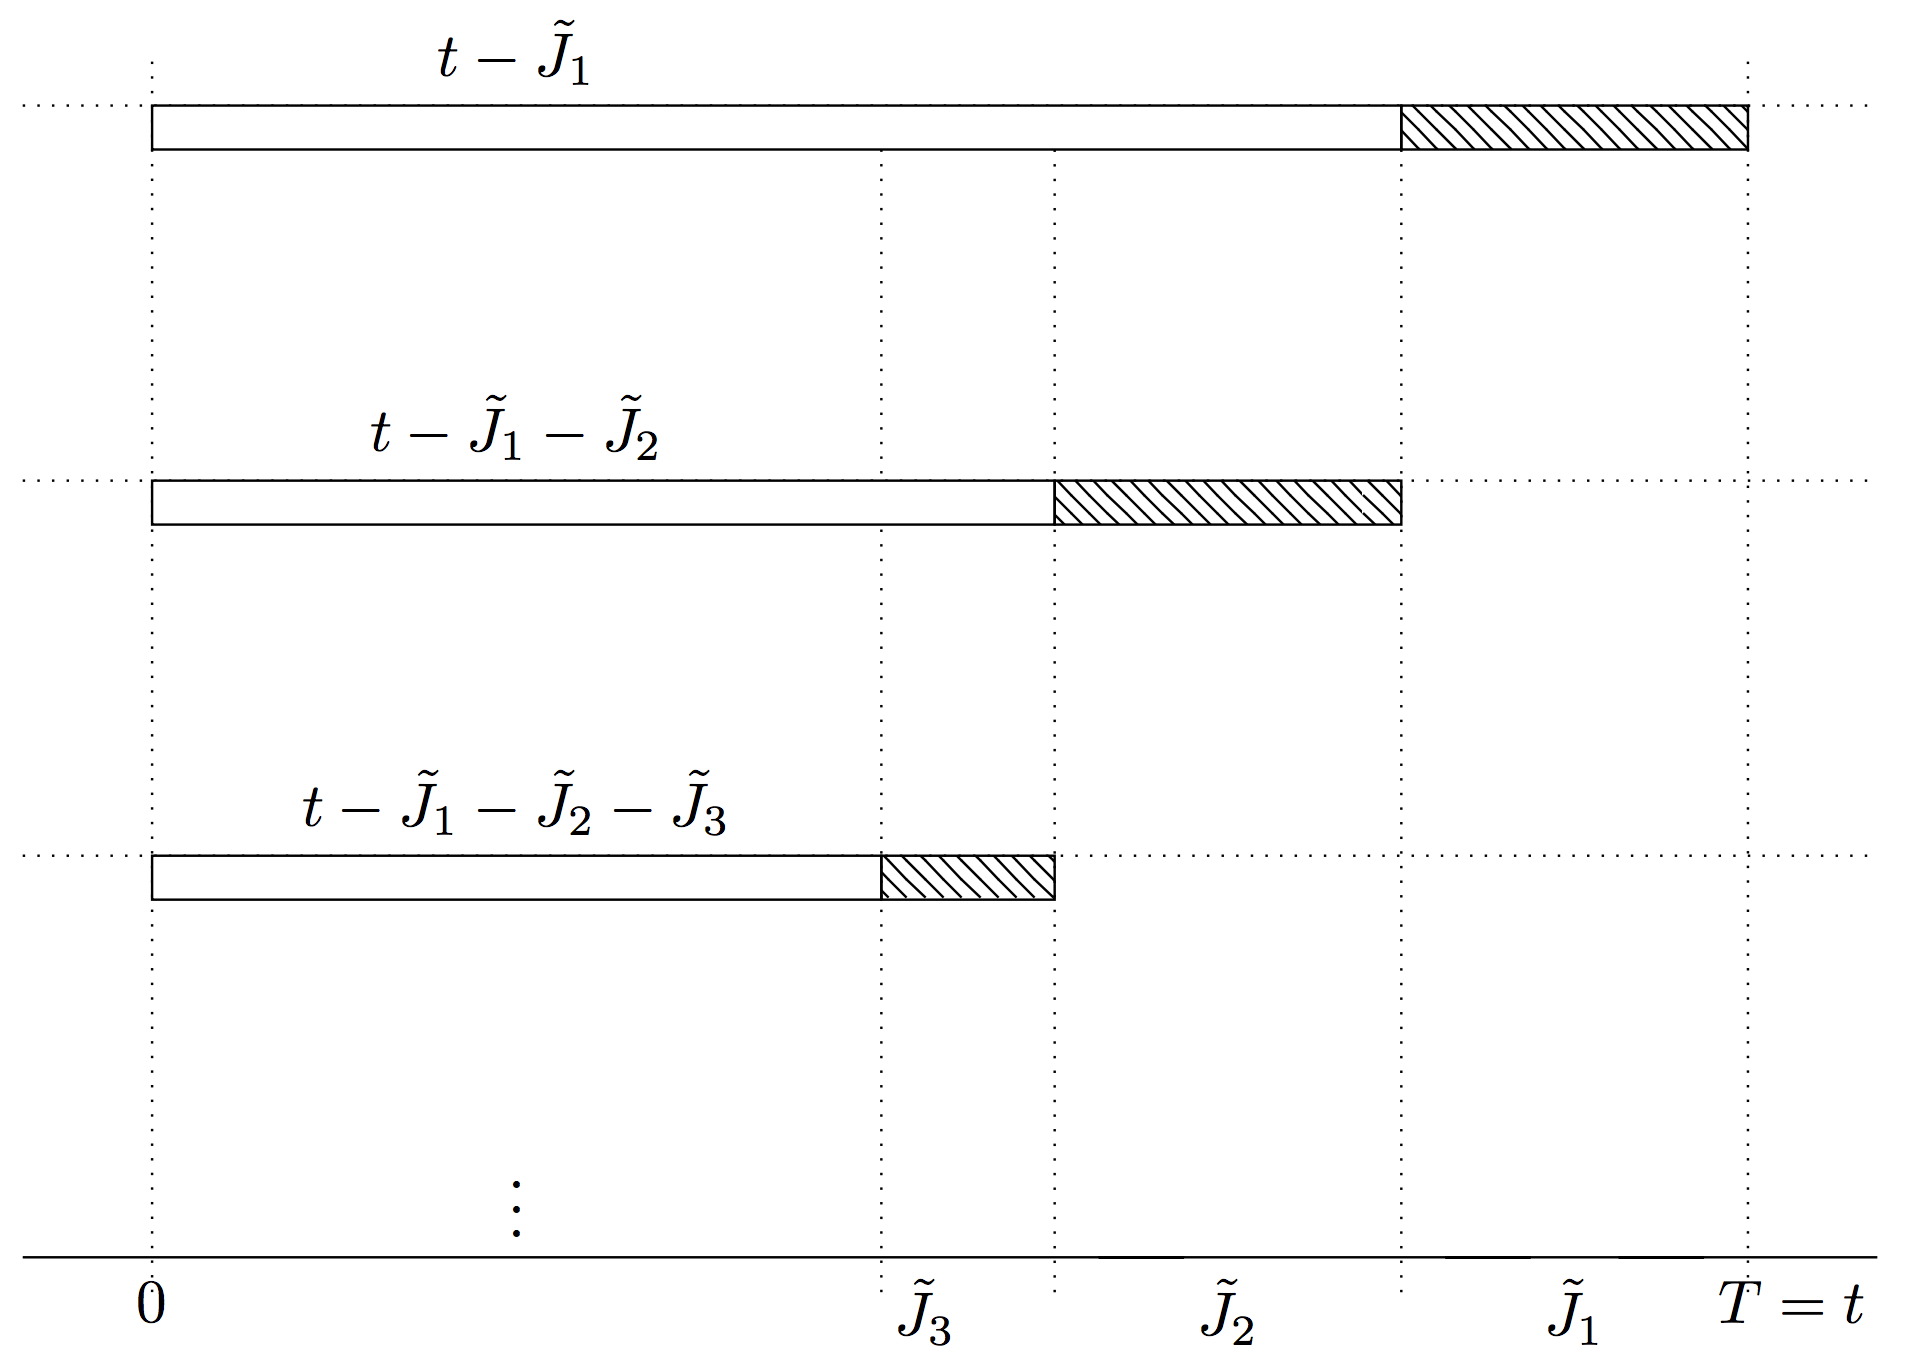
\includegraphics[width=\textwidth]{PK_generative_process2.png}
    \caption{Generative process of Poisson-Kingman Process. Source: \cite{LomeliThesis}.}
  \end{minipage}
  \hfill
  \begin{minipage}[b]{0.48\textwidth}
    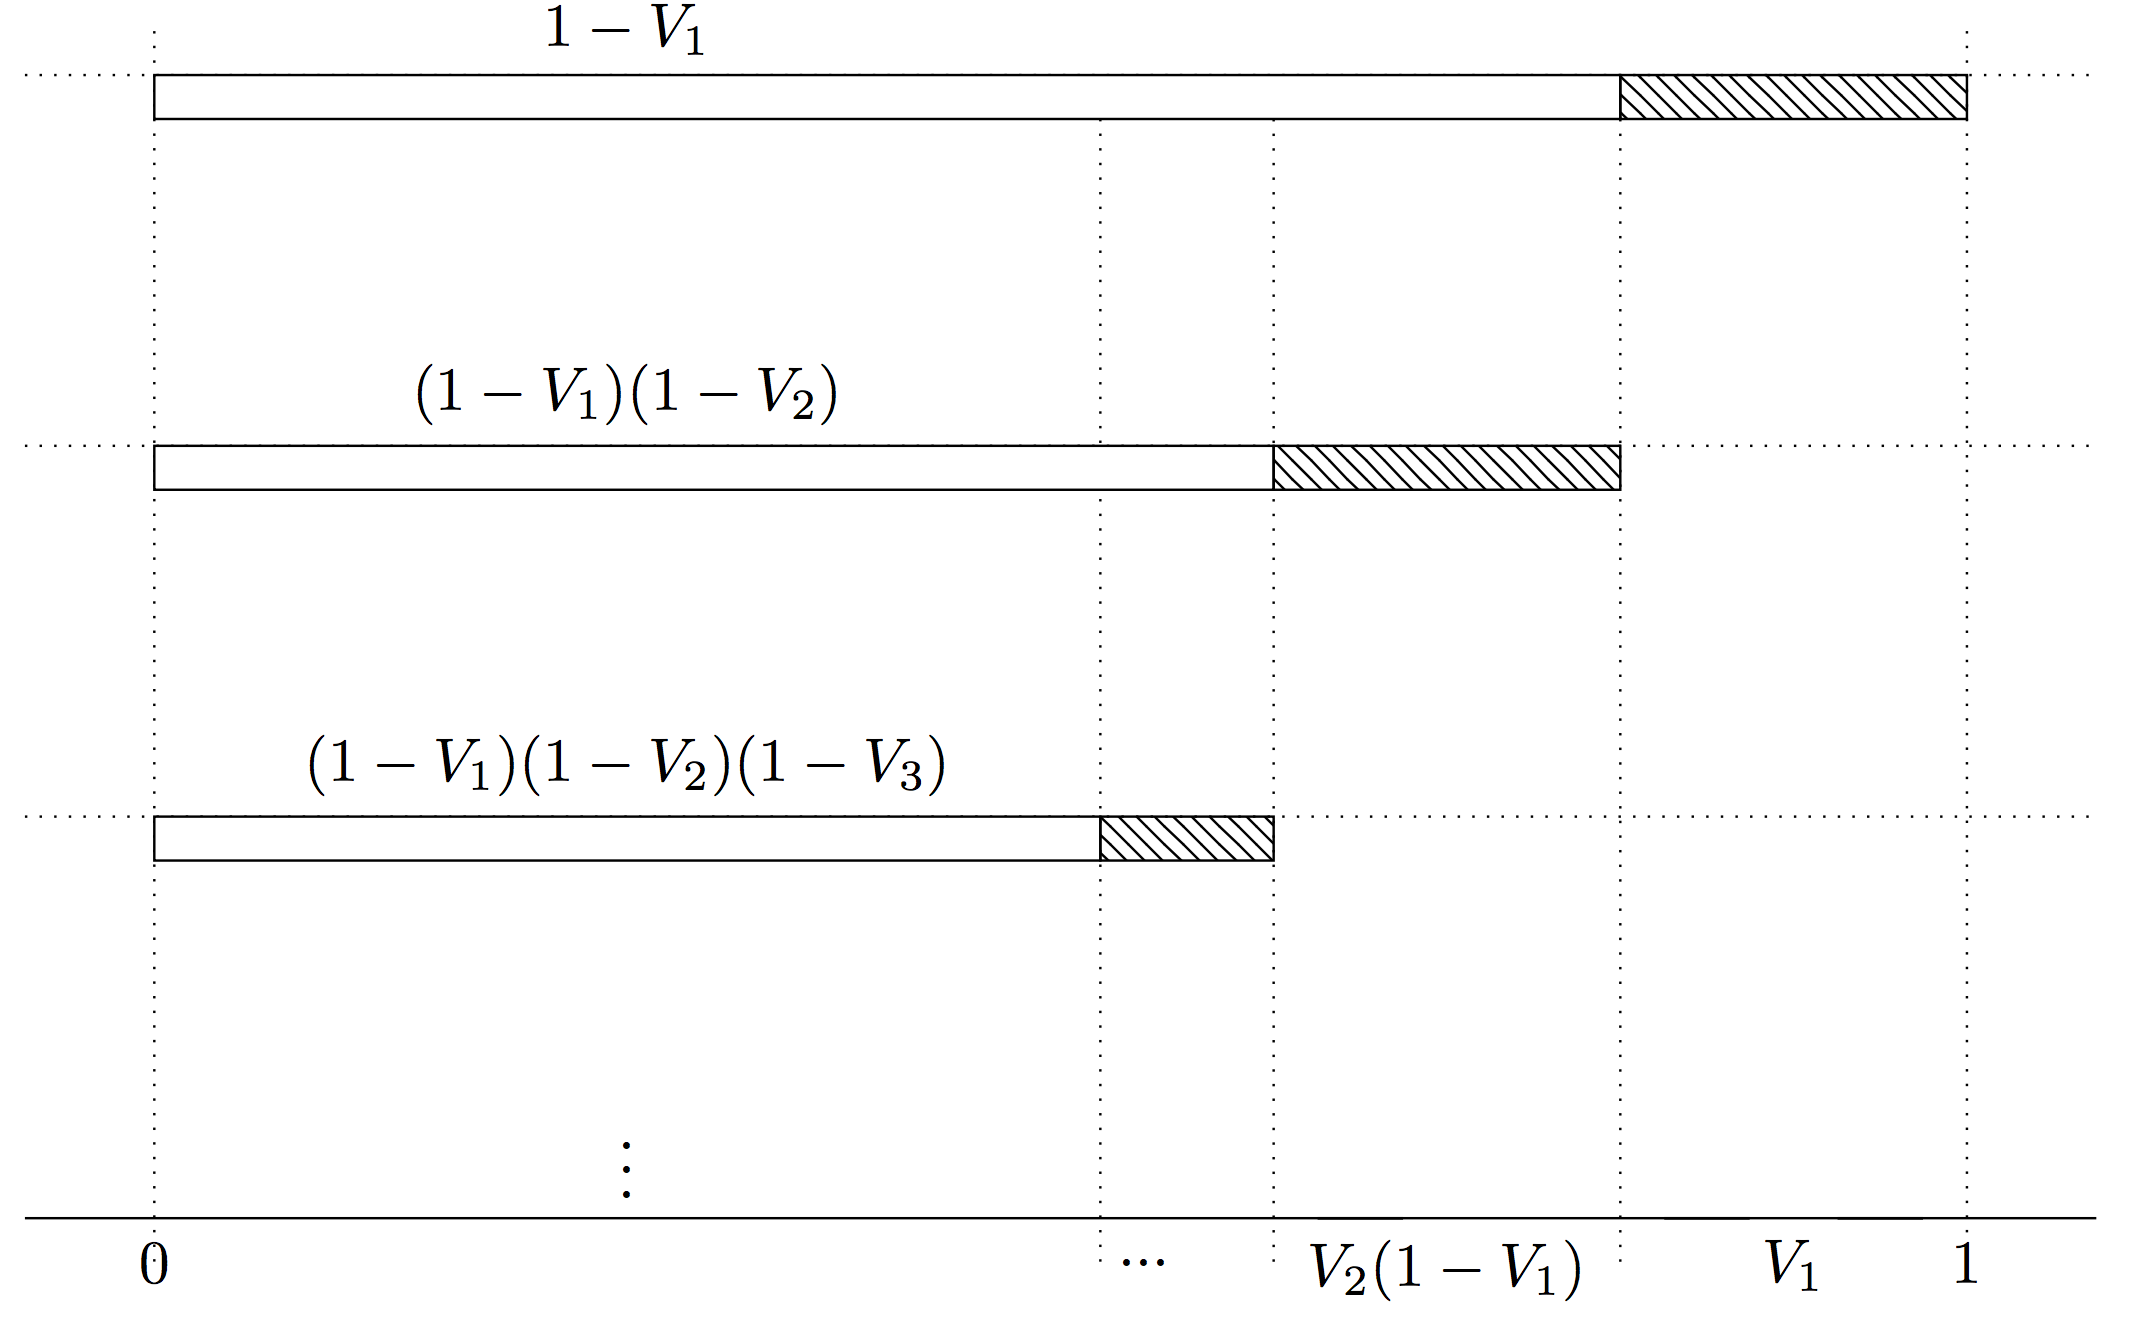
\includegraphics[width=\textwidth]{PY_stick_breaking2.png}
    \caption{Stick-breaking construction. Source: \cite{LomeliThesis}.}
  \end{minipage}
\end{figure}

we reviewed the PKP generative process from Figure \ref{fig:PK_generative_process}, it is reminiscent of the well-known stick breaking construction from \ref{sethuraman94}, where a stick of length one is broken, as in Figure \ref{fig:PY_stick_breaking}, but it is not the same. As mentioned previously, we can reparameterise the model, starting with Equation (2.24), and obtain the corresponding joint distribution in terms of $N$ $(0,1)$-valued stick-breaking weights $\{\tilde{p}_j \}_{j=1}^N$, where $N$ is the number of represented sticks after trunctation (Favaro and Walker, 2012). This joint distribution is for a general Lévy measure $\rho$, density $f_\rho$ and it is conditioned on the valued of the random variable $T$. We can then recover the well-known Stick breaking representations for the Dirichlet and Pitman-Yor processes, for a specific choice of $\rho$, if we integrate out $T$.

However, in general, these stick random variables, denoted by $V_l := \frac{\tilde{p}_l}{1 - \sum_{i<l}{\tilde{p}_l}}$ form a sequence of dependent random variables with a complicated distribution, except for the two previously mentioned processes, see Pitman (1996) for details.

\begin{gather*}
T \sim \gamma \\
\tilde{J}_1|T \sim \text{SBS}(T) \\
\tilde{J}_2|T,\tilde{J}_1 \sim \text{SBS}(T - \tilde{J}_1) \\
\vdots \\
\tilde{J}_{l}|T,\tilde{J}_1,\dots,\tilde{J}_{l-1} \sim \text{SBS}(T - \sum_{i<l} \tilde{J}_i) \\
\vdots \\
\end{gather*}
the corresponding weights are:
$$ \tilde{p}_k := \frac{\tilde{J}_{k}}{T_k} = \frac{\tilde{J}_{k}}{T - \sum_{j=1}^{k-1} \tilde{J}_j} $$


Cf meeting with Ben
$\beta_i = \frac{\tilde{J}_i}{T_{i-1}}$
$\tilde{p_i} = \beta_i \prod_{j=1}^i (1-\beta_i)$


\section{Models of interest}
calculus for SMC for BNP mixture with fixed parameters
fixed parameters are not a assumption, since can be made random then with PMCMC


Ultimately we would like to define a distribution on an infinite set of discrete outcomes that will represent our categories or mixture components, but we start by defining a distribution on the natural numbers.
Use Homogeneous assumption, when a new $(X_k^\star)$

\begin{lstlisting}[caption={\acrlong{DP} written in Julia.},captionpos=b,label=code:DP]
function DP($\alpha$, $H_0$) =    begin
  augmentedProc = @memoize (stickIndex) -> rand($H_0$)
  DP = makeSticks($\alpha$)
  return () -> augmentedProc(DP())
end
\end{lstlisting}


The code of the \gls{DP} stick-breaking process and of the infinite mixture model which has been used for our experiments can be found here: \url{link} \textcolor{red}{ADD LINK}.

\begin{lstlisting}[caption={Nonconjugate infinite mixture model written in Turing.jl.},captionpos=b,label=code:IMM]
@model InfiniteMixutre(y) = begin
  N = length(y)
  $\alpha$ =  10.0
  m ~ Normal(meanMean, 1.0/sqrt(meanPrecision)) # Assume statement
  s ~ Gamma(precisionShape, 1.0/precisionInvScale) # Assume statement
  P = rand(DP($\alpha$, Normal(m, 1.0/sqrt(s)))) # Random probability measure

  x = tzeros(N)
  for i in 1:N
    x[i] ~ P # Assume statement
    y[i] ~ Normal(x[i], 1.0/sqrt(s)) # Observe statement
  end

  return x
end
\end{lstlisting}

Note the use of the \texttt{for-loop} so as to express the model as \acrlong{SSM}. Such a formulation will indeed allow us to make use of particle algorithms (described in Subsections \ref{IS} and \ref{PMCMC}).

\section{Sampler}
Now that we have detailed and implemented a generative process (i.e. sampling from the prior) for our class of models, we focus in this section on the sampler scheme to use within the \gls{PPL}.

\textcolor{red}{paper reference for particle methods for high dimensional space}
%It has been shown that particle methods are the class of sampler scheme to use in the case of high dimensional space.
%\gls{SMC} for 
We are interested in the more general Bayesian case were the parameters are also random variables and to be inferred. Consequently, \acrlong{PMCMC} are methods of choice.

Yet, there is a big path degeneracy issue. The first $X_t$s ($t$ close to $1$) have way lower \gls{ESS} compared to $X_t$s at the end of the sequence. This is a well-known issue, which is tackled in \gls{PGAS} and \gls{IPMCMC}.

\gls{PMMH} should bring symmetry in the \gls{ESS} graph (\gls{ESS} for the $y$-axis and $t$ index for the $x$-axis), i.e. all $X_t$s should have in average the same \gls{ESS}.

We believe that \gls{PGAS} is not suited with \gls{BNP} models since ...
This is the reason why I am currently working on the implementation of \gls{IPMCMC} for Turing.

\section{Experimentations}

\textcolor{red}{Sampling from -logBeta PKP}

\textcolor{red}{Posterior distribution of hyperparmeters for DP mixture}

\textcolor{red}{Posterior distribution of mixture components for DP mixture, highlight path degeneracy}

\section{Open questions}
Some questions are still open on this subject, and we are currently working on these.

Is a stick-breaking-like Markov Chain necessary and sufficient for doing inference with particle methods?

What should be the representation of the state in the PPL (theoretically and efficiently concerned) ?

$(\{X_j^\star\}_{j=1}^k, \{z_i\}_{i=1}^N)$ or $\{X_i\}_{i=1}^N$
where $N$ the total number of observations, $k$ is the number of different component, $\{X_j^\star\}_{j=1}^k$ the (unique) mixture components, and $\{z_i\}_{i=1}^N$ the individual assignments.

Should we include the sticks lengths (weights) $\{\tilde{J}_j\}_{j=1}^k$

Other models than infinite mixture models  
